% Generated by code/needham.py -- do not edit by hand.
\definecolor{qocA}{rgb}{0.00,0.45,0.70}
\definecolor{qocB}{rgb}{0.90,0.60,0.00}
\definecolor{qocC}{rgb}{0.00,0.62,0.45}
\definecolor{qocD}{rgb}{0.80,0.40,0.00}
\definecolor{qocE}{rgb}{0.80,0.60,0.70}
\definecolor{qocF}{rgb}{0.35,0.70,0.90}
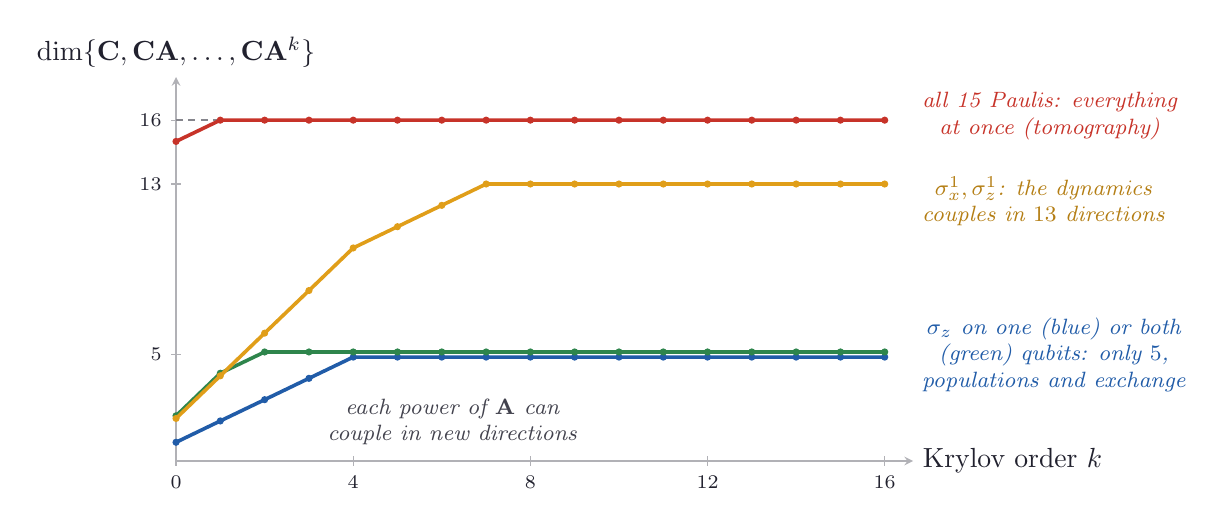
\begin{tikzpicture}[ink/.style={line width=0.9pt, ndInk}, faint/.style={line width=0.4pt, ndInk!35}, dashedink/.style={line width=0.5pt, ndInk!55, dash pattern=on 2.5pt off 2pt}, vec/.style={->, >=stealth, line width=1.2pt}, note/.style={font=\footnotesize\itshape, text=ndInk!85, align=center}, pointer/.style={->, >=stealth, line width=0.4pt, ndInk!60, shorten >=2pt, shorten <=1pt}, dot/.style={circle, fill=ndInk, inner sep=0pt, minimum size=3.4pt}, wash/.style={fill=ndSky, fill opacity=0.55}, every node/.style={text=ndInk}]
\definecolor{ndInk}{rgb}{0.13,0.13,0.18}
\definecolor{ndPaper}{rgb}{0.99,0.96,0.88}
\definecolor{ndSky}{rgb}{0.84,0.91,0.98}
\definecolor{ndRose}{rgb}{0.98,0.86,0.84}
\definecolor{ndBlue}{rgb}{0.13,0.36,0.66}
\definecolor{ndRed}{rgb}{0.78,0.20,0.16}
\definecolor{ndGold}{rgb}{0.88,0.62,0.10}
\definecolor{ndGreen}{rgb}{0.18,0.52,0.30}
\draw[faint, ->, >=stealth] (0.000,0.000) -- (9.360,0.000) node[right, text=ndInk] {Krylov order $k$};
\draw[faint, ->, >=stealth] (0.000,0.000) -- (0.000,4.876) node[above, text=ndInk] {$\dim\linspan\{\mathbf C,\mathbf C\mathbf A,\dots,\mathbf C\mathbf A^k\}$};
\draw[faint] (0.000,0.060) -- (0.000,-0.060) node[below, font=\scriptsize, text=ndInk] {$0$};
\draw[faint] (2.250,0.060) -- (2.250,-0.060) node[below, font=\scriptsize, text=ndInk] {$4$};
\draw[faint] (4.500,0.060) -- (4.500,-0.060) node[below, font=\scriptsize, text=ndInk] {$8$};
\draw[faint] (6.750,0.060) -- (6.750,-0.060) node[below, font=\scriptsize, text=ndInk] {$12$};
\draw[faint] (9.000,0.060) -- (9.000,-0.060) node[below, font=\scriptsize, text=ndInk] {$16$};
\draw[faint] (0.060,1.353) -- (-0.060,1.353) node[left, font=\scriptsize, text=ndInk] {$5$};
\draw[faint] (0.060,3.518) -- (-0.060,3.518) node[left, font=\scriptsize, text=ndInk] {$13$};
\draw[faint] (0.060,4.329) -- (-0.060,4.329) node[left, font=\scriptsize, text=ndInk] {$16$};
\draw[dashedink] (0.000,4.329) -- (9.000,4.329);
\draw[line width=1.3pt, ndBlue] (0.000,0.238) -- (0.562,0.509) -- (1.125,0.779) -- (1.688,1.050) -- (2.250,1.320) -- (2.812,1.320) -- (3.375,1.320) -- (3.938,1.320) -- (4.500,1.320) -- (5.062,1.320) -- (5.625,1.320) -- (6.188,1.320) -- (6.750,1.320) -- (7.312,1.320) -- (7.875,1.320) -- (8.438,1.320) -- (9.000,1.320);
\fill[ndBlue] (0.000,0.238) circle (1.3pt);
\fill[ndBlue] (0.562,0.509) circle (1.3pt);
\fill[ndBlue] (1.125,0.779) circle (1.3pt);
\fill[ndBlue] (1.688,1.050) circle (1.3pt);
\fill[ndBlue] (2.250,1.320) circle (1.3pt);
\fill[ndBlue] (2.812,1.320) circle (1.3pt);
\fill[ndBlue] (3.375,1.320) circle (1.3pt);
\fill[ndBlue] (3.938,1.320) circle (1.3pt);
\fill[ndBlue] (4.500,1.320) circle (1.3pt);
\fill[ndBlue] (5.062,1.320) circle (1.3pt);
\fill[ndBlue] (5.625,1.320) circle (1.3pt);
\fill[ndBlue] (6.188,1.320) circle (1.3pt);
\fill[ndBlue] (6.750,1.320) circle (1.3pt);
\fill[ndBlue] (7.312,1.320) circle (1.3pt);
\fill[ndBlue] (7.875,1.320) circle (1.3pt);
\fill[ndBlue] (8.438,1.320) circle (1.3pt);
\fill[ndBlue] (9.000,1.320) circle (1.3pt);
\draw[line width=1.3pt, ndGreen] (0.000,0.574) -- (0.562,1.115) -- (1.125,1.385) -- (1.688,1.385) -- (2.250,1.385) -- (2.812,1.385) -- (3.375,1.385) -- (3.938,1.385) -- (4.500,1.385) -- (5.062,1.385) -- (5.625,1.385) -- (6.188,1.385) -- (6.750,1.385) -- (7.312,1.385) -- (7.875,1.385) -- (8.438,1.385) -- (9.000,1.385);
\fill[ndGreen] (0.000,0.574) circle (1.3pt);
\fill[ndGreen] (0.562,1.115) circle (1.3pt);
\fill[ndGreen] (1.125,1.385) circle (1.3pt);
\fill[ndGreen] (1.688,1.385) circle (1.3pt);
\fill[ndGreen] (2.250,1.385) circle (1.3pt);
\fill[ndGreen] (2.812,1.385) circle (1.3pt);
\fill[ndGreen] (3.375,1.385) circle (1.3pt);
\fill[ndGreen] (3.938,1.385) circle (1.3pt);
\fill[ndGreen] (4.500,1.385) circle (1.3pt);
\fill[ndGreen] (5.062,1.385) circle (1.3pt);
\fill[ndGreen] (5.625,1.385) circle (1.3pt);
\fill[ndGreen] (6.188,1.385) circle (1.3pt);
\fill[ndGreen] (6.750,1.385) circle (1.3pt);
\fill[ndGreen] (7.312,1.385) circle (1.3pt);
\fill[ndGreen] (7.875,1.385) circle (1.3pt);
\fill[ndGreen] (8.438,1.385) circle (1.3pt);
\fill[ndGreen] (9.000,1.385) circle (1.3pt);
\draw[line width=1.3pt, ndGold] (0.000,0.541) -- (0.562,1.082) -- (1.125,1.624) -- (1.688,2.165) -- (2.250,2.706) -- (2.812,2.976) -- (3.375,3.247) -- (3.938,3.518) -- (4.500,3.518) -- (5.062,3.518) -- (5.625,3.518) -- (6.188,3.518) -- (6.750,3.518) -- (7.312,3.518) -- (7.875,3.518) -- (8.438,3.518) -- (9.000,3.518);
\fill[ndGold] (0.000,0.541) circle (1.3pt);
\fill[ndGold] (0.562,1.082) circle (1.3pt);
\fill[ndGold] (1.125,1.624) circle (1.3pt);
\fill[ndGold] (1.688,2.165) circle (1.3pt);
\fill[ndGold] (2.250,2.706) circle (1.3pt);
\fill[ndGold] (2.812,2.976) circle (1.3pt);
\fill[ndGold] (3.375,3.247) circle (1.3pt);
\fill[ndGold] (3.938,3.518) circle (1.3pt);
\fill[ndGold] (4.500,3.518) circle (1.3pt);
\fill[ndGold] (5.062,3.518) circle (1.3pt);
\fill[ndGold] (5.625,3.518) circle (1.3pt);
\fill[ndGold] (6.188,3.518) circle (1.3pt);
\fill[ndGold] (6.750,3.518) circle (1.3pt);
\fill[ndGold] (7.312,3.518) circle (1.3pt);
\fill[ndGold] (7.875,3.518) circle (1.3pt);
\fill[ndGold] (8.438,3.518) circle (1.3pt);
\fill[ndGold] (9.000,3.518) circle (1.3pt);
\draw[line width=1.3pt, ndRed] (0.000,4.059) -- (0.562,4.329) -- (1.125,4.329) -- (1.688,4.329) -- (2.250,4.329) -- (2.812,4.329) -- (3.375,4.329) -- (3.938,4.329) -- (4.500,4.329) -- (5.062,4.329) -- (5.625,4.329) -- (6.188,4.329) -- (6.750,4.329) -- (7.312,4.329) -- (7.875,4.329) -- (8.438,4.329) -- (9.000,4.329);
\fill[ndRed] (0.000,4.059) circle (1.3pt);
\fill[ndRed] (0.562,4.329) circle (1.3pt);
\fill[ndRed] (1.125,4.329) circle (1.3pt);
\fill[ndRed] (1.688,4.329) circle (1.3pt);
\fill[ndRed] (2.250,4.329) circle (1.3pt);
\fill[ndRed] (2.812,4.329) circle (1.3pt);
\fill[ndRed] (3.375,4.329) circle (1.3pt);
\fill[ndRed] (3.938,4.329) circle (1.3pt);
\fill[ndRed] (4.500,4.329) circle (1.3pt);
\fill[ndRed] (5.062,4.329) circle (1.3pt);
\fill[ndRed] (5.625,4.329) circle (1.3pt);
\fill[ndRed] (6.188,4.329) circle (1.3pt);
\fill[ndRed] (6.750,4.329) circle (1.3pt);
\fill[ndRed] (7.312,4.329) circle (1.3pt);
\fill[ndRed] (7.875,4.329) circle (1.3pt);
\fill[ndRed] (8.438,4.329) circle (1.3pt);
\fill[ndRed] (9.000,4.329) circle (1.3pt);
\node[note, anchor=west, text=ndRed] at (9.35,4.38) {all 15 Paulis: everything\\ at once (tomography)};
\node[note, anchor=west, text=ndGold!80!black] at (9.35,3.30) {$\sigma_x^1,\sigma_z^1$: the dynamics\\ couples in $13$ directions};
\node[note, anchor=west, text=ndBlue] at (9.35,1.35) {$\sigma_z$ on one (blue) or both\\ (green) qubits: only $5$,\\ populations and exchange};
\node[note, anchor=south west] at (1.800,0.081) {each power of $\mathbf A$ can\\ couple in new directions};
\end{tikzpicture}
